\section{MiG-23}

\noindent
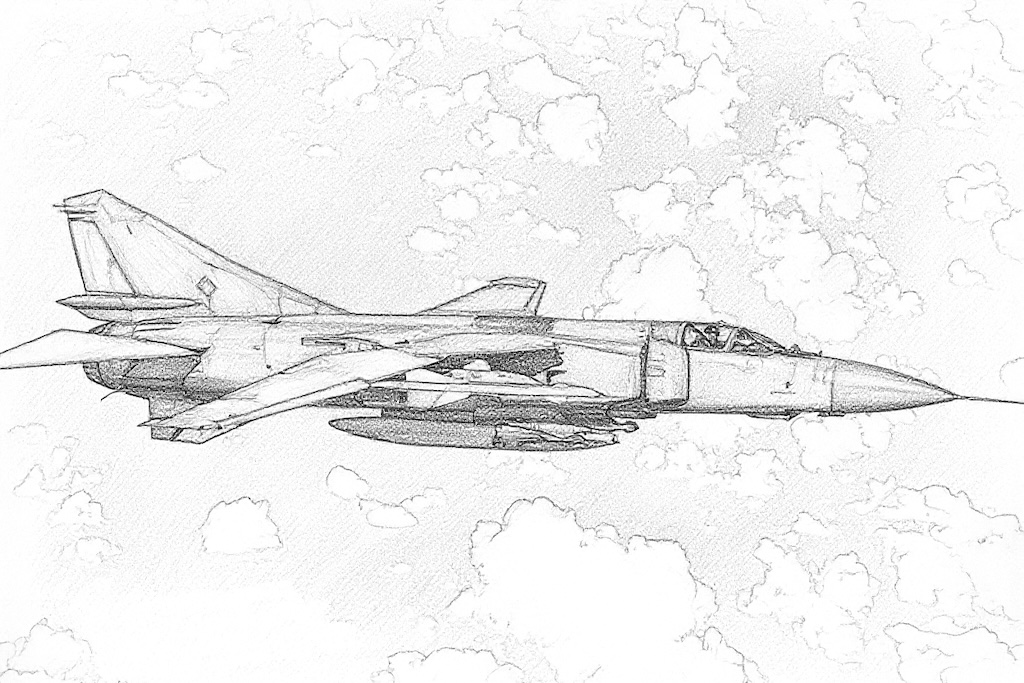
\includegraphics[width=\linewidth]{MiG-23.jpg}

\noindent
The Mikoyan-Gurevich MiG-23 is a single-seat fighter, interceptor, and ground-attack aircraft. It is single-engined, supersonic, and variable-geometry wings, and is notably more complex than the MiG-21 it was designed to replace. Mature versions are armed with a look-down/shoot-down radar and long-range air-to-air missiles.

Ground-attack versions were developed from the fighter versions, and later developed into the specialized MiG-27 aircraft.
%
\note{Sources}{

    \begin{itemize}
        \item Alexander Mladenov, Soviet Cold War Fighters, 2016 (Fonthill).
        \item Greg Goebel, \href{https://airvectors.net/avmig23_1.html}{Air Vectors} (Wayback)
        \item \href{https://en.wikipedia.org/wiki/Mikoyan-Gurevich_MiG-23}{Wikipedia on the MiG-23}
        \item \href{https://en.wikipedia.org/wiki/List_of_MiG-23_operators}{Wikipedia on MiG-23 operators}
        \item \href{https://en.wikipedia.org/wiki/Gryazev-Shipunov_GSh-23}{Wikipedia on the GSh-23L}
        \item \href{https://en.wikipedia.org/wiki/Kh-23_Grom}{Wikipedia on the Kh-23 (AS-7 Kerry)}
        \item \href{http://www.jbg37.de/html/bewaffnung.html}{MiG-23BN loads on JBG-27 site}
    \end{itemize}

    \noteparagraph{Source ADCs}
    \begin{itemize}
        \item {\AirSup}: MiG-23MF Flogger-G.
        \item {\EOTG}: MiG-23BN Flogger-F.
        \item {\APJ} 12: MiG-23BN Flogger-F.
        \item {\APJ} 39: MiG-23MS Flogger-E.
        \item {\APJ} 43: MiG-23M/MF Flogger-B.
        \item {\APJ} 44: MiG-23M/MF Flogger-B.
        \item Chris Perleberg: MiG-23M/MS Flogger-B/E.
        \item Felix Hack: MiG-23M/MF apparently from {\APJ} 44.
        \item Malcolm Pipes: MiG-23M/MF Flogger-B, MiG-23MS Flogger-E, MiG-23ML/MLA/P Flogger-G, MiG-23MLD Flogger-K, and MiG-23BN/BK Flogger F/H
    \end{itemize}

    \noteparagraph{Photo Credit}
    \begin{itemize}
        \item \href{https://commons.wikimedia.org/wiki/File:Mig-23-DNST8908431_JPG.jpg}{DoD} (Public Domain)
    \end{itemize}
}

\subsection{Versions}

\begin{table*}
    \centering
    \caption*{MiG-23 Version and Variant Summary}
    \footnotesize
    \begin{tabularx}{0.9\linewidth}{lcccL}
        \toprule
        Version (Variant)&NATO&In&ADC&Notes\\
        &Subtype&Service\\
        \midrule
        MiG-23S&A&1970&N&Initial version with \emph{Edition 1} wings, with leading-edge slats, and with the RP-22SM Sapfir-21 (Jay Bird) radar. Able to use only R-3/R-13 (AA-2A/B/C) AAMs. No external FTs.\\
        MiG-23&&1971&N&Improved version of the MiG-23S with larger \emph{Edition 2} wings without leading-edge slats, the Sapfir-23L (High Lark) radar without look-down, and an IRST. Able to use R-23 (AA-7A/B) AAMs of the same type and R-3/R-13 (AA-2A/C) IRMs. Centerline FT, but no wing FTs.\\
        MiG-23M&B&1973&Y&Improved version of the MiG-23 with \emph{Edition 3} wings leading-edge slats, with the Sapfir-23D radar with limited look-down, and also able to use R-60 (AA-8) IRMs. Centerline and wing FTs.\\
        MiG-23MS&F&1974&Y&Export version based on the MiG-23M, but with the RP-22SM Sapfir-21 (Jay Bird) radar and no IRST. Able to use only R-3/R-13 (AA-2A/B/C) AAMs, and with degraded ECM.\\
        MiG-23ML&G&1976&Y&Improved version of the MiG-23M, with a lightened airframe, more powerful engine, and the Sapfir-23ML radar with full look-down. Able to use R-23 (AA-7A/B) AAMs of different types simultaneously.\\
        MiG-23MF (Warsaw Pact)&B&1978&Y&Export version of the MiG-23M very similar to the base version.\\
        MiG-23MF (Export)&B&1978&Y&Export version of the MiG-23M with degraded radar and ECM.\\
        MiG-23MLA&G&1978&Y&Improved version of the MiG-23ML, with a very similar airframe but improved Sapfir-23MLA radar. Able to carry the R-24 (AA-7C/D) AAM.\\
        MiG-23MLA (Warsaw Pact)&G&1981&Y&Export version of the MiG-23MLA very similar to the base version.\\
        MiG-23MLA (Export)&G&1981&Y&Export version of the MiG-23MLA with degraded radar and ECM.\\
        MiG-23P&G&1979&Y&Interceptor versionfor the PVO derived from the MiG-23ML.\\
        MiG-23MLD\\
        MiG-23B\\
        MiG-23BM\\
        \bottomrule
    \end{tabularx}
\end{table*}

\subsubsection{MiG-23S}

The MiG-23S is the initial production fighter version. Its NATO reporting name is Flogger-A.%
\note{MiG-23S Technical Data}{
    See Mladenov, Goebel, and Wikipedia on the MiG-23. I do not propose to provide an ADC for this version

    \noteparagraph{Fuel} Mladenov gives fuel tank capacities that sum to 4,250 liters.

}

It is equipped with the R-27F-300 or R-27F2-300 engine and early \emph{Edition 1} wings with leading- and trailing-edge flaps for better take-off and landing performance. The wings can be set to a forward position for low-speed flight, a middle position for a balance of speed and maneuverability, and a rear position for high-speed flight.

Because of delays in the development of the RP-23 Sapfir-23 radar, the MiG-23S is equipped with the RP-22SM Sapfir-21 (Jay Bird) radar from MiG-21S/SM.
It also lacks the IRST and HUD of later versions.

In addition to the internal 23~mm GSh-23L cannon, it has two stations under the wing gloves and two more under the fuselage for R-3S or R-13M (AA-2A/C Atoll) IRMs, R-3R (AA-2B Atoll) RHMs, or air-to-ground ordnance including the Kh-23 (AA-7 Kerry) RG.

As the Soviet Union's first swing-wing combat aircraft, the MiG-23S represented a step-change in complexity for manufacturers, maintainers, and flight crew, and suffered from reliability problems. The most serious defects were cracks in the airframe, which limited it to 4G, and a propensity to enter a spin at a high angle-of-attack.

Only about 60 MiG-23S were built. They entered service with VVS in 1970, but were soon withdrawn.%
\note{MiG-23S Service History}{
    See Mladenov, Goebel, and Wikipedia on the MiG-23.
}

\subsubsection{MiG-23}

The MiG-23 (also known unofficially as the MiG-23 \emph{Edition 1971}) is an iteration of the MiG-23S.%
\note{MiG-23 Technical Data}{
    See Mladenov, Goebel, and Wikipedia on the MiG-23. I do not propose to provide an ADC for this version.

    \noteparagraph{Fuel} Mladenov states an additional fuel tank was added, giving a total capacity of 4,720 liters. This is 404 fuel points at 6.5 lb/gal and 20 lb/point. I have changed the ADC to have 400 fuel points.

}

It continues to use the R-27F2-300 engine of later MiG-23S aircraft, but has a modified fuselage with the tail surfaces moved to the rear and \emph{Edition 2} wings with 20\% greater area but without flaps.

The MiG-23 is equipped with the Sapfir-23L (High Lark A) radar which is a great improvement on the Sapfir-21 radar of the MiG-23S, but in this version lacks a look-down/shoot-down capability.
It is also equipped with an IRST and HUD.

Its principal armament is a pair of R-23R RHMs or R-23T IRMs (AA-7A/B Apex), but only one kind can be carried on each mission.
The secondary armament is a pair of R-3S or R-13M (AA-2A/C Atoll) IRMs.

The changes in the airframe did not resolve the dangerous behavior at high angle-of-attack or doubts about its ability to survive more than 4G.

Only about 80 MiG-23 were built. They entered service with VVS-FA in 1971, but were transferred to a training role in 1978.%
\note{MiG-23 Service History}{
    See Mladenov, Goebel, and Wikipedia on the MiG-23.
}

\subsubsection{MiG-23M}

The MiG-23M is the first version that saw large-scale production and service.
Its NATO reporting name is Flogger-B.%
\note{MiG-23M ADC and Technical Data}{
    See Mladenov, Goebel, and Wikipedia on the MiG-23.

    The ADC is based on the one in {\APJ} 43/44; this was the latest one published for a version of the MiG-23 in {\APJ} and so presumably represents the best estimation of its performance.

    I have made the following modifications:
    \begin{itemize}
        \item Power and fuel consumption taken from Malcolm Pipe's ADC. The {\APJ} 43/44 has a fuel consumption of 2.5 in N power, which is anomalous.
        \item Radar and ECM taken from Malcolm Pipe's ADC.
        \item Auto-track technology taken from Malcolm Pipe's ADC.
        \item I follow Malcolm Pipe's in noting that sources differ on whether the DDS and AJM were actually fitted.
        \item The wing and centerline station loads were increased to 1,730 lb to be able to carry the 800L FT.
    \end{itemize}

}

It is powered by an improved R-29-300 engine, capable of 18,400~lb of dry thrust and 25,500~lb with afterburner. The wings were changed again, and these \emph{Edition 3} wings retaining the greater area of those of the MiG-23 but regaining leading-edge slats for improved performance on take-off and landing. The new wings also have two fixed stations for 800L FTs, the use of which requires the wings to remain in the forward position until the FTs and pylons are jettisoned.

The MiG-23M is equipped with the Safir-23D (High Lark II) radar (later upgraded to the Safir-23D-III), with a limited look-down/shoot-down capability.

Its armament options are similar to the those of the MiG-23, but it also gained the capability to use R-60/60M (AA-8 Aphid) IRMs.

The MiG-23M entered service with the VVS in 1973 and the IA PVO in the mid 1970s.%
\note{MiG-23M Service History}{
    See Mladenov, Goebel, and Wikipedia on the MiG-23M.
}

Manufacturing problems persisted, and until 1977 the MiG-23M was limited to 5G. In combat, this limit would of course have been ignored, but the pilots would have found themselves unaccustomed to the effects of high-G and more susceptible to GLOC; in the game this is reflected in a \minus{1} modifier for GLOC rolls.

\subsubsection{MiG-23MS}

The MiG-23MS is a downgraded export version derived from the MiG-23M, with much of the sensitive modern avionics replaced with older equivalents.
Its NATO reporting name is Flogger-F.%
\note{MiG-23MS ADC and Technical Data}{
    See Mladenov, Goebel, and Wikipedia on the MiG-23. The ADC is largely based on the 23M with radar from the MiG-21S and ECM from the MiG-23MF Export variant. The HUD Interface is from Malcolm Pipes' ADC.
}

The RP-22SM (Jay Bird) radar, previously used in the MiG-21S and MiG-23S, replaces the Sapfir-23L, and so the MiG-23MS uses the less effective R-3R/R-3S/R-13S (AA-2A/B/C Atoll) AAMs rather than the R-23R/T (AA-7A/B Apex) AAMs. The IRST and ECM equipment are also removed.
The airframe and engine of the MiG-23MS are almost identical to those of the MiG-23M, except that the nose cone is shorter as the RP-23SM radar is more compact.

The MiG-23MS was manufactured from 1973 to 1978, and served in the air forces of Afghanistan (from 1988), Algeria, Democratic Republic of Congo, Egypt (from 1974), Iraq (from 1974), Libya (from 1974), Sudan (from 1987), and Syria (from October 1973).%
\note{MiG-23MS Service History}{
    See Mladenov, Goebel, and Wikipedia on the MiG-23 and its operators.
}

The MiG-23MS undoubtedly suffered the same maneuvering restrictions as the MiG-23M, and also will have a \minus{1} modifier for GLOC rolls.

\subsubsection{MiG-23ML}

The MiG-23ML is an improved version of the MiG-23M.
Its NATO reporting name is Flogger-G.%
\note{MiG-23ML ADC and Technical Data}{
    See Mladenov, Goebel, and Wikipedia on the MiG-23.
    The ADC is based on the ADC by Malcolm Pipes.

    \noteparagraph{Fuel} Mladenov states that the No.\ 4 fuel tank (470L) was removed, which would give a total internal capacity of 4,250 lb or 363 fuel points (at 6.5 lb/gal and 20 lb/point). I have changed the internal fuel capacity to 365 fuel points.

    \noteparagraph{Fuel Consumption} Mladenov notes that its specific fuel use was 93\% of that of the 23M in full afterburner, but its thrust is 106\% larger, and these two factors even out to give it the same fuel consumption as the 23M. I have modified the ADC accordingly.
}

The MiG-23ML has a redesigned and lightened fuselage, a more powerful R-35F-300 engine, with 18,850~lb of dry thrust and 28,800~lb of afterburner thrust. The airframe is strengthened and does not suffer from the robustness problems that plagued earlier version. These improvements give significantly better performance than the MiG-23M. The avionics are also improved. The internal fuel capacity is slightly reduced.

The Sapfir-23ML radar has a considerably improved look-down/shoot-down capability compared to the previous Sapfir-23D-III. Additionally, both the R-23R RHM and the R-23T IRM can be employed on the same mission. The IRSTS is improved too.

The MiG-23ML was manufactured from 1975 to 1977. It entered service with the VVS in 1976.%
\note{MiG-23ML Service History}{
    See Mladenov, Goebel, and Wikipedia on the MiG-23.
}

\subsubsection{MiG-23MF}

The MiG-23MF is a second export version derived from the MiG-23M.
Its NATO reporting name is Flogger-B.

The airframe and engine of the MiG-23MF are identical to the MiG-23M.
The Sapfir-23D-III radar is also retained, but is redesignated as Sapfir-23E, as is the capability to use R-23R/T (AA-7 Apex) AAMs.
However, in terms of avionics and weapons, there are two major variants.
The Warsaw Pact variant is almost identical to the MiG-23M.
The Export variant has degraded ECCM for the radar and other avionics, and was only supplied with the R-60 (AA-8 Aphid) IRM starting in 1981.%
\note{MiG-23MF ADC and Technical Data}{
    See Mladenov, Goebel, and Wikipedia on the MiG-23. The ADC is largely based on the 23M.

    \noteparagraph{Warsaw Pact Variant} The Warsaw Pact variant is identical to the MiG-23M.

    \noteparagraph{Export Variant} The Export variant has degraded radar ECM/ECCM (which I take to be a radar ECCM of 0, no auto-track, RWR-A instead of B, and no AJM), no datalink, and the R-60 only from 1981. The degraded ECM/ECCM and the radar is largely taken Malcolm Pipes' ADC.

}

The MiG-23MF was manufactured from 1978 to 1983.
The Warsaw Pact variant served in the air forces of Bulgaria, Czechoslovakia, East Germany, Hungary, Poland, and Romania, and the Export variant served in the air forces of Algeria (from 1982), Cuba (from 1984), India (from 1980), Iraq (from 1981), Libya (from 1984), and Syria (from 1978).%
\note{MiG-23MF Service History}{
    See Mladenov, Goebel, and Wikipedia on the MiG-23.
}

\subsubsection{MiG-23MLA}

The MiG-23MLA is an improved version of the MiG-23ML.
Its NATO reporting name is Flogger-G.%
\note{MiG-23MLA ADC and Technical Data}{
    See Mladenov, Goebel, and Wikipedia on the MiG-23.
    The ADC is based on the ADC by Malcolm Pipes.

    I am assuming that the Export version has ECCM of zero and RWR-A only.

}

The airframe of the MiG-23MLA is identical to that of the MiG-23ML, but the radar, gunsight, and missile systems are significantly improved. The Sapfir-23MLA radar has better range, reliability, ECM, and avoids mutual interference. The longer-ranged and more lethal R-24R/T (AA-7C/D Apex) AAMs can be carried.

The Warsaw Pact variant is very similar to the base variant for the VVS. The export variant has downgraded radar and ECM.

The MiG-23MLA was manufactured from 1977 to 1983 and entered service with the VVS in 1978. The Warsaw Pact version entered service with the air forces of Bulgaria, Czechoslovakia, and East Germany in 1981. The export version entered service with the air forces of Angola, Cuba, Iraq, North Korea, and Yemen in the early 1980s.%
\note{MiG-23ML Service History}{
    See Mladenov, Goebel, and Wikipedia on the MiG-23.
}

\subsubsection{MiG-23P}

The MiG-23P is a derivative of the MiG-23ML optimized as an interceptor for the PVO.
Its NATO reporting name is Flogger-G.%
\note{MiG-23MLA ADC and Technical Data}{
    See Mladenov, Goebel, and Wikipedia on the MiG-23.
    The ADC is based on the ADC by Malcolm Pipes.

    \noteparagraph{IRSTS} Pipes' ADC specifies that the MiG-23P does not have an IRSTS. However, Mladenov states that externally it was identical to the MiG-23ML/MLA except for the antennas on the fin tip and that the IRSTS for the MiG-23PD were adapted from MiG-23P/ML. Also, images on MiG-23Ps show the IRSTS housing under the nose. All of this suggests that the MiG-23P did indeed retain the IRSTS of the ML.

}

The airframe and engine are identical to the MiG-23ML, but the radar and other avionics are adapted to PVO standards and specialized for its duty as an interceptor.

The MiG-23P was manufactured from 1978 to 1981 and entered service with the PVO probably in 1979. %
\note{MiG-23ML Service History}{
    See Mladenov, Goebel, and Wikipedia on the MiG-23.
}

\subsubsection{MiG-23MLD}

The MiG-23MLD is an improved version of the MiG-23MLA. Its NATO reporting name is Flogger-K and Flogger-G.%
\note{MiG-23MLD ADC and Technical Data}{
    See Mladenov, Goebel, and Wikipedia on the MiG-23.
    The ADC is based on the ADC by Malcolm Pipes.

    I am not sure how to handle the improvements in high angle-of-attack behavior. Perhaps previous version have a chance of a maneuvering departure if they use the ET rate and this version does not?

    \noteparagraph{DDS} Mladenov reports that MLD has a pair of six-round chaff/flare dispensers installed in the centerline pylon and a pair of thirty-round chaff/flare dispensers on the upper rear fuselage. (It is not clear if previous versions has any DDS.) The total number of rounds would be 72 and so the number of clusters would be 18--36 (at the stated rate of 2--4 rounds per cluster). This seems to be a DDS-B.

}

The version for VVS has modifications to the airframe to improve its handling at high angle-of-attack. An additional wing position of 33 degrees (between the forward and mid positions of 16 and 45 degrees) is available, although it was not widely used. Additionally, the radar, weapons systems, and ECM systems are improved. All the VVS MiG-23MLDs were converted from in-service MiG-23MLAs.

The version for export has the improvements to the radar, weapons systems, and ECM systems, but does not have the improvements to the airframe.

The MiG-23MLD entered service with the VVS in 1982. The export variant entered service with the air forces of Syria (in 1982) and Bulgaria (in 1983).

\subsubsection{MiG-23B}

The MiG-23B is the original strike version. Its NATO reporting name is Flogger-F.
It first flew in 1971.
Changes from the interceptor version include the AL-21F engine with 17,200 lbf of dry thrust and 24,700 lbf of afterburner thrust, the second-edition wing with greater area but no leading-edge flaps, additional armor, more robust landing gear, more fuel, and two additional weapon stations on the rear fuselage.
It retains the GSh-23L cannon of the MiG-23.
The air-to-air radar and the original nose are replaced with a laser tracker and a navigation radar in a low-profile nose that gives much better forward visibility.
A Siren-FSh jammer and a Siren-10M RMR are installed.%
\note{MiG-23B Technical Data}{
    See Wikipedia and Goebel.

    \noteparagraph{Load} The total load is 3,000~kg (Goebel).

    \noteparagraph{Fuel} The internal fuel was increased to 1,517 US gallons (Goebel).

}

Only about two dozen MiG-23B were built.
It entered service in the VVS-FA probably in 1971 or 1972, but was not exported as the AL-21F was restricted to Soviet use.%
\note{MiG-23B Service and Combat}{
    See Wikipedia and Goebel.
}

\subsubsection{MiG-23BN}

The MiG-23BN is based on the MiG-23B, but has an R-29B-300  engine with 17,310 lbf of dry thrust and 23,370 lbf of afterburner thrust, the third-edition wings (with greater area and leading-edge flaps), and other minor changes.
Its NATO reporting name is Flogger-H.
The R-29 engine was available in larger numbers than the AL-21F of the MiG-23B (which was largely reserved for the Su-17 and Su-24) and was also authorized for export. It was first striker version to be produced in larger numbers.%
\note{MiG-23BN Technical Data}{
    See Wikipedia, Goebel, and JBG-27 site.

    The initial ADC is based on that of the MiG-27. In terms of flight characteristics, this is not especially realistic because of the difference in intake geometry; it would be better to base the flight characteristics on an early MiG-23.
}

About six hundred MiG-23BN were built, and they served in the Soviet VVS-FA from 1973 and with the air forces of Bulgaria, Czechoslovakia, and East Germany.
An export variant, without countermeasure equipment and with degraded avionics, served in the air forces of Algeria, Cuba, Egypt, Ethiopia, India, Iraq, Libya, and Syria.%
\note{MiG-23BN Service and Combat}{
    See Wikipedia and Goebel.
}

\subsection{Armament and Stores}

\paragraph{Gun}\note{Gun}{See Wikipedia on the MiG-23 and GSh-23.
    A GSh-23L has a rate of fire of 3,500 rounds per minute, so 200 rounds corresponds to 1.7 ammunition points.
}
All MiG-23 versions are armed with a 23~mm GSh-23L gun with 200 rounds.%

\paragraph{Loads and Stations}
The initial MiG-23S has only four weapon stations, two under the fuselage and two under the wing gloves, and can carry 2,000~kg (4,400~lb) of external stores. The MiG-23 gains a centerline station for an FT. The MiG-23M gains wing stations for FTs, and can carry 3,000~kg (6,600~kg) of external stores.%
\note{Loads and Stations}{
    \begin{itemize}
        \item MiG-23S can carry total load of 2,000~kg or 4,400~lb and has only the wing-glove and fuselage station (Mladenov and Goebel).
        \item MiG-23M can carry total load of 3,000~kg or 6,600~lb and also has the centerline or wing stations (Mladenov and Goebel). I presume the MiG-23MF is identical in these respects. The ADCs for these vary from 5,500~lb to 7,750~lb.
        \item MiG-23BN can carry 6,600 lb (3,000 kg) (Goebel and on the JGB-37 site)

    \end{itemize}

    The fixed wing stations of the 23M/23BN are described by Goebel and confirmed by the JBG-37 site. If they only carry an 800L FT, then the maximum weight on them will be 1,730~lb.

    The maximum weight on the wing-glove and fuselage stations of the 23M is 1,100~lb according to Perleberg's ADC.

    The maximum weight on the MiG-23BN wing-glove stations is 2,200 lb (two FAB-500 in tandem) according to the JBG-37 site. The maximum weight on the MiG-27 wing-glove stations is 2,400 lb (four FAB-250 on an MR) according to Goebel. The {\AirStr} and Perleberg ADCs allow a load of only 1,500 lb.

    The maximum weight on the MiG-23BN forward fuselage stations is 1,200 lb (four FAB-100 on a MR) according to the JBG-37 site. The maximum weight on the MiG-27 forward fuselage stations is 1,200 lb (two FAB-250 on a DR) according to Goebel. The {\AirStr} and Perleberg ADCs allow a load of only 1,100 lb.

    The maximum weight on the rear fuselage stations is 550 lb (one FAB-250) according to Goebel.

    We can see that the heaviest loads (and hence minimum load capacities) on the stations are:
    \begin{itemize}
        \item Wing stations (1 and 9): 1,730 lb for the 800L FT.
        \item Wing-glove stations (2 and 8): 2,300 lb for two FAB-500 BBs on a DR.
        \item Forward-fuselage stations (3 and 7): 1,100 lb for one FAB-500 BB.
        \item Rear-fuselage stations (4 and 6): 550 lb for one FAB-250 BB.
        \item Centerline station (5): 1,730 lb for the 800L FT.
    \end{itemize}
}

\paragraph{Fuel Tanks}
The initial MiG-23S has no provision for external fuel tanks, but all later versions can carry an 800L FT on a centerline station and all versions from the MiG-23M can also carry two 800L FTs on the wing stations provided the wings are in the forward position.%
\note{Fuel Tanks}{
    See Goebel and Mladenov.
}

\paragraph{Gun Pods}
The MiG-23ML/MLA/MLD can carry UPK-23-250 23~mm gun pods on the wing-glove stations.%
\note{Gun Pods}{
    Mladenov states that the ability to carry the UPK-23-250 GP was added to the MiG-23ML; the MiG-23S/23/23M/23MF do not have this capacity.
}

\paragraph{Air-to-Air Weapons}
The MiG-23S/MS, with their older radar and fire-control systems derived from the MiG-21S, can only carry R-3S/R-3R/R-13M (AA-2A/B/C Atoll) AAMs.

The radar-less MiG-23B/BN can only carry R-3S/R-13M (AA-2A/C Atoll) IRMs singly and R-60/60M (AA-8 Aphid) IRMs either singly or in pairs on MDRs.

All other versions can carry R-23R/T (AA-7A/B Apex) AAMs singly on the wing-glove stations, but the MiG-23/23M/MF can only carry either two RHMs or two IRMs and cannot mix an RHM with an IRM, and the R-3S or R-13M IRMs on the fuselage stations. The MiG-23MLA can carry the improved R-24R/T (AA-7C/D Apex) AAMs from 1981. They can also carry R-3S/R-13M (AA-2A/C Atoll) IRMs singly and R-60/60M (AA-8 Aphid) IRMs either singly or in pairs on MDRs.%
\note{Air-to-Air Weapons}{
    See Mladenov and Goebel.

    Wikipedia on the R-23 states that the R-24 was used by Syria, Iraq, Angola, presumably by MiG-23MLA (Export).

}

\paragraph{Air-to-Ground Weapons}%
\note{Air-to-Ground Weapons}{
    See Mladenov and Goebel.

    \noteparagraph{MiG-23M/MF/MS}
    By comparison with the MiG-23BM, I suggest the following possible air-to-ground loads:
    \begin{itemize}
        \item One 800L FT on CL (1,730 lb).
        \item One 800L FT on CL and two 800L FT on the wing stations (5,190 lb).
        \item One 800L FT on CL and four UB-16-57 RPs on the fuselage and wing-glove stations (2,930 lb).
        \item Four S-24 rockets on fuselage and wing-glove stations (2,000 lb).
        \item Sixteen FAB-100 and four MRs on the fuselage and wing-glove stations (4,320 lb).
        \item Four FAB-250s on the wing-glove stations and fuselage station (4,400 lb).
        \item One 800L FT on CL and two FAB-500 BBs on the wing-glove stations (3,930 lb).
        \item One 800L FT on CL and four FAB-500 BBs on the wing-glove and fuselage stations (6,130 lb)
        \item One 800L FT on CL and two K-23 (AS-7) RGs on the wing-glove stations (2,990 lb)
        \item One RN-40 NBB on the left fuselage station (550 lb).
    \end{itemize}

    \noteparagraph{MiG-23ML} UPK-23-250 can be carried on the wing-glove stations (Mladenov).

    \noteparagraph{MiG-23BN Stations and Loads}

    The loads on the JGB-37 site are:
    \begin{itemize}
        \item One 800L FT on CL (1,730 lb).
        \item One 800L FT on CL and two 800L FT on wing stations (5,190 lb).
        \item One 800L FT on CL and four UB-16-57/UB-32 RPs on forward-fuselage and wing-glove stations (3,730 lb).
        \item One 800L FT on CL and two B-8M1 RPs (\binarymultiply{20}{85~mm}) RPs (each 500 lb?) on wing-glove stations (2,730 lb).
        \item Four S-24 rockets on forward-fuselage and wing-glove stations (2,000 lb).
        \item One 800L FT on CL and two UPK-23-250 GPs on the wing-glove stations (2,730 lb).
        \item Sixteen FAB-100 and four MRs on the forward-fuselage and wing-glove stations and two FAB-100s on the rear-fuselage stations (4,760 lb).
        \item Four FAB-250s and two DRs on the wing-glove stations and four more on the forward-fuselage and rear-fuselage stations (4,600 lb).
        \item One 800L FT on CL and four FAB-500 BBs on two DRs on the wing-glove stations (6,330 lb).
        \item One 800L FT on CL and four FAB-500 BBs on the wing-glove and forward-fuselage stations (6,130 lb)
        \item One 800L FT on CL and two K-23 (AS-7) RGs on the wing-glove stations (2,990 lb)
        \item Two 800L FTs on the wing stations, four FAB-500 BBs on two DRs on the wing-glove stations and two B-8M1 RPs (\binarymultiply{20}{85~mm}) RPs (each 500 lb?) on the forward-fuselage stations (9,060 lb). the last configuration has a weight of 9.060 lb. Without the FTs, it would be 5,600 lb, and that seems more reasonable.
        \item One RN-40 NBB on the left forward-fuselage station (550 lb). This is labelled with “Russian variant”, presumably because nuclear weapons were not issued to DDR forces.
    \end{itemize}
Goebel also mentions Iraqi MiG-23BMs carrying French ATLIS DP for Kh-29L (AS-14 Kedge) RGs and \binarymultiply{5}{122~mm} RPs.}
Despite being designed as a fighter, the MiG-23S/23/23/M have a significant ait-to-ground capability and can carry FAB-100/250/500 BBs, ZAB-500 incendiary BBs, and RBK-500 cluster BBs, UB-16-57 (\binarymultiply{16}{57~mm}) RPs, S-24 (240 mm) RKs, and Kh-23 (AS-7 Kerry) RGs.
The MiG-23M can also carry a single RN-24 or RN-40 nuclear BB on its left fuselage station.

\subsection{ADCs}

ADCs are provided for:
\begin{adclist}
    \adcitem{MiG-23M}
    \adcitem{MiG-23MS}
    \adcitem{MiG-23ML}
    \adcitem{MiG-23MF (Warsaw Pact)}
    \adcitem{MiG-23MF (Export)}
    \adcitem{MiG-23MLA}
    \adcitem{MiG-23MLA (Warsaw Pact)}
    \adcitem{MiG-23MLA (Export)}
    \adcitem{MiG-23P}
    \adcitem{MiG-23BN}
\end{adclist}

\listofnotes
